\dictum[Zizek]{Something about what is good.}

\begin{summary}
\item FluiDB is well suited for join-heavy star schemata so we
  evaluated using the SSB-TPC-H benchmark.
\item Our evaluation shows that FluiDB is able to plan around the
  space constraints and come up with plans that materialize
  intermediate results that are useful for future queries.
\item FluiDB is generally faster than the baseline due to caching but
  at times may be slower when it receives ``unexpected''
  queries.
\item FluiDB generally performs better when allowed larger memory
  budgets but this speedup is based on heuristic assumptiosn that
  sometimes break in interesting ways.
\end{summary}

We based our evaluation on the Star Schema Benchmarkx (SSB)
\cite{barataOverviewDecisionSupport2015} which is a variation of
TPC-H. Like TPC-H it models the data warehouse of a wholesale
supplier. It is organized in four "flights" (groups):

\begin{itemize}
\item The first flight performs a single join between the Lineorder table
and the small Date dimension table.
\item Queries in Flight 2 join the Lineorder, Date, Part and Supplier
tables. They aggregate and sort data on Year and Brand.
\item Starting from a specific customer, supplier, region and date, flight
3 selects into specific cities and years.
\item Flight 4 is the most complex one, as it joins all tables.
\end{itemize}

Each flight contains 3 queries making a total of 12 distinct queries.

As the name suggests these queries query a star schama. The star
schema is derived from the TPC-H schema (figure \ref{fig:tpch_schema})
by merging the \sql{linenumber}, \sql{orders} and
\sql{partsupp} and completely dropped tables \sql{nation} and
\sql{region} tables as shown in figure \ref{fig:ssb_tpch_schame}.

\begin{figure}[p]
\begin{tikzdiagram}
  \tikzset{tbl/.style={draw,rectangle,minimum height=2cm,minimum width=2cm}};
  \node[tbl] (lo) {lineorder};
  \node[tbl] (p) [above left = of lo] {part};
  \node[tbl] (c) [above right = of lo] {customer};
  \node[tbl] (s) [below right = of lo] {supplier};
  \node[tbl] (d) [below left = of lo] {date};
  \draw [-stealth] (c) -- (lo);
  \draw [-stealth] (p) -- (lo);
  \draw [-stealth] (s) -- (lo);
  \draw [-stealth] (d) -- (lo);
\end{tikzdiagram}
\caption{\label{fig:ssb_tpch_schema}The foreign key links in a SSB-TPC-H}
\end{figure}


\begin{figure}[p]
\begin{tikzdiagram}
  \tikzset{tbl/.style={draw,rectangle,minimum height=2cm,minimum width=2cm}};
  \tikzset{arr/.style={-stealth}};
  \node[tbl]                     (r) {region};
  \node[tbl, right=of r]         (n) {nation};
  \node[tbl, above right = of n] (c) {customer};
  \node[tbl, right = of n] (s) {supplier};
  \node[tbl, right = of c]         (o) {orders};
  \node[tbl, right=of s]         (ps) {partsupp};
  \node[tbl, below left = of ps] (p) {part};
  \node[tbl, right= of ps]        (l) {lineitem};
  % Connection
  \path [arr]
  (r) edge (n)
  (n) edge (c)
  (c) edge (o)
  (o) edge (l)
  (n) edge (s)
  (s) edge (ps)
  (ps) edge (l)
  (p) edge (ps);
\end{tikzdiagram}
\caption{\label{fig:tpch_schema}The foreign key links in a traditional TPC-H schema}
\end{figure}


The particular queries contained in the workload are presented in
listing [ref] in the appendix (\ref{chapter:appendix}).

We generated a workload where queries were compiled and planned one by
one in a loop for and run them over a database of data generated with
a modified version of the TPC-H dbgen
\cite{perivolaropoulosFakedrakeSsbdbgen2021a} with scaling of size 1,
meaning that the total primary data is around 1GB in CSV format. The
exact size of the data generated after formatting them to the format
required by FluiDB (described in chapter \ref{chapter:execution}) are

\begin{minted}[]{sh}
$ du -sh *.dat
4.1M    customer.dat
256K    date.dat
757M    lineorder.dat
31M     part.dat
268K    supplier.dat
\end{minted}

Which makes a total of approximately 200k pages.

The lowset budget within which FluiDB was able to plan all 12 queries
of SSB-TPC-H was 2200k pages.

In our expriment we use page IO as a proxy for performance, despite
the fact that FluiDB is an in-memory database. We think that this is a
reasonable experimental approach because, as FluiDB leans heavily on
code generation, it is unlikely that the actual intruction retiring
will have a major impact on the perofrmance. Instead the perfomance
cost is dominated by page IO that will certainly cause cache misses at
the LLC. Another thing to note is that FluiDB generates code that
focuses on performance and not on compilation time, making heavy use
of metaprogramming like \cpp{constexpr} and temlpates.  This makes for
fairly slow compilation times (approximately 1 sec to 2 sec with
\texttt{-O2}). There are ways to speed up compilation time like using
pre-compiling header files \cite{PrecompiledHeadersPCH} and
fine-tuning the compiler optimization passes. These techniques are
beyond the scope of this work, FluiDB is focused on analytics
workloads that do not include sub-second queries.

\begin{figure}[p]
\centering
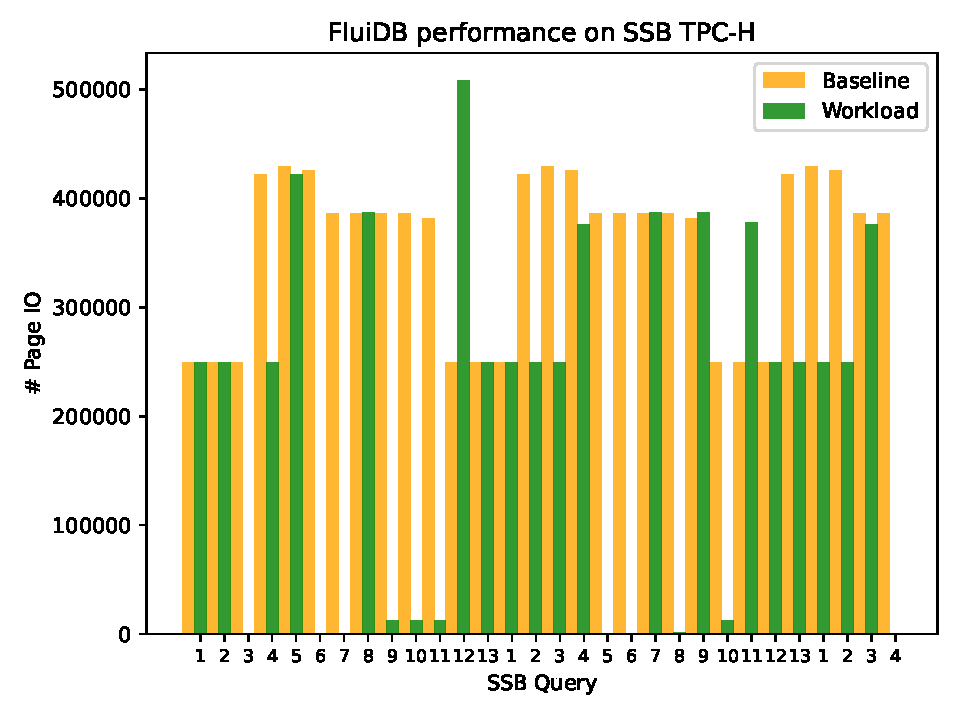
\includegraphics[width=.9\linewidth]{./plans/io_perf_22000.pdf}
\caption{\label{fig:min_budget_plot}
  The total page read/writes for each query a sequence of queries. The
  SSB query number is \(mod(\text{query sequence},12\). The baseline
  is the query being run by FluiDB directly without any materialized
  nodes. The workload bars represent the cost of each query in a
  workload built within the same QDAG. The budget for this is the
  minimum budget within which FluiDB can run each individual query.}
\end{figure}

It is clear from figure \ref{fig:min_budget_plot} that even at the minimum budget
FluiDB is able to come up with an efficient plan at every case. In
some cases, however the garbage collector is forced to delete tables
that need to be recreated causing FluiDB to be sporadically less
performant than the base case.

For a larger budget the FluiDB is able to store more useful
intermediate results as demonstrated in figure \ref{fig:large_budget_plot}

\begin{figure}[p]
\centering
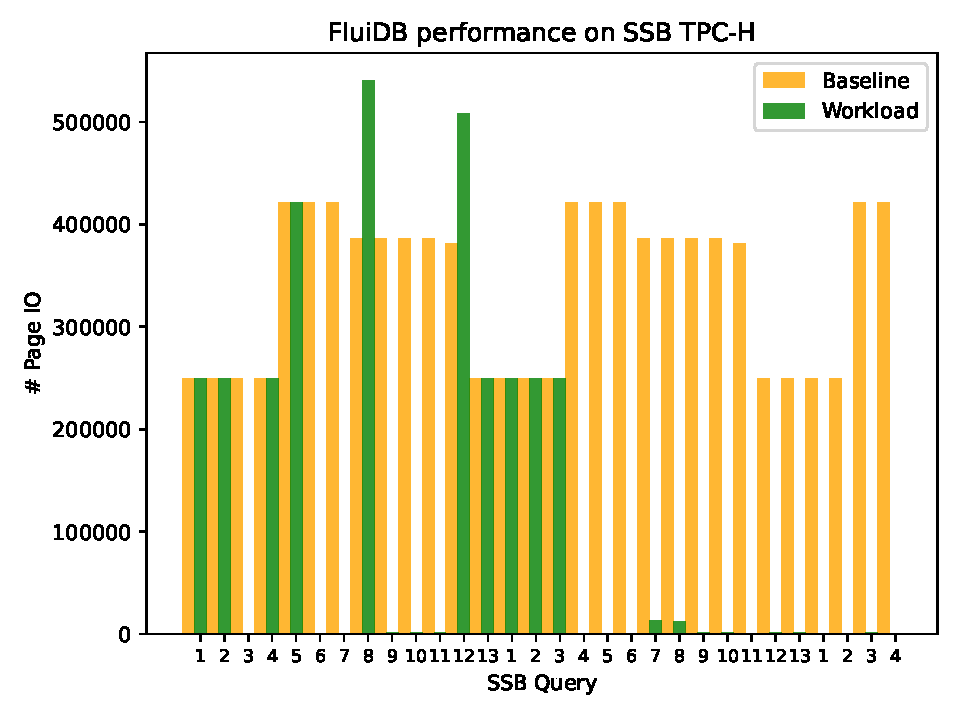
\includegraphics[width=.9\linewidth]{./plans/io_perf_60000.pdf}

\caption{\label{fig:large_budget_plot}
  The total page read/writes for each query a sequence of queries. The
  SSB query number is \(mod(\text{query sequence},12)\). The baseline
  is the query being run by FluiDB directly without any materialized
  nodes. The workload bars represent the cost of each query in a
  workload built within the same QDAG. The budget for this is triple
  the minimum budget within which FluiDB can run each individual
  query.}
\end{figure}

An interesting point here is the plan for evaluating query 8 is more
expensive in the workload run under laxer budgetary constraints. This is strange

The top level explanation is that the lax-budget plan needs to
evaluate \(\mathit{lineorder}\) via the reverse trigger of a join as
it was deleted during evaluation of query 7. Mysteriously during the
strict-budget planning the \(\mathit{lineorder}\) relation is readily
available during planning of query 8! The key is slightly earlier in
the workload. FluiDB, materializes in query 5 all the join

\[
Q := \mathit{supplier} \Join_{\mathit{lo\_suppkey} = \mathit{s\_suppkey}} \mathit{lineorder}
\]

and corresponding antijoins \(Q_1\) and \(Q_2\) making the node
\(\mathit{lineorder})\) deletable. However, when running the workload
under strict budgetary constraints, it is forced to garbage collect
shortly after materializing said join at a moment while both \(Q\) and
\(\mathit{lineorder})\) are protected (see section \ref{sec:gc} on
garbage collection). Therefore, FluiDB is forced to delete both
\(Q_1\) and \(Q_2\). This makes \(\mathit{lineorder})\) non-deletable
when planning for query 5 finishes.

On the other hand, whith laxer budgetary constraints, no garbage
collection is triggered during query 5. In fact the next garbage
collection is triggered during query 7, at a moment when
\(\mathit{lineorder})\) is deletable, unprotected, and a prime
candidate for deletion based on the GC heuristics.

Alas, when query 8 requires \(\mathit{lineorder})\) for its plan,
FluiDB needs to re-construct it in the case of lax budgetary
constraints but, not in the case of strict constraints.

This example of FluiDB being force to locally produce more expensive
plans is an of FluiDB being more opportunistic the lower the available
budget is, and more adventurous when operating with high budgets. When
FluiDB is frugal it is generally prone to miss oportunities to share
computation between queries. There are times however that this
fugality saves it from bad heuristic-based decisions that it is
allowed to make otherwise.

FluiDB aspires to deal with the entire workload as if it were planning
a single query. While any decision during the planning of a single
query can be undone, FluiDB is tragically forced to commit to whatever
adveturous or conservative decisions it makes at the end of every
planning iteration, doomed to pay dearly for every misstep but to reap
the rewards of every insightful choice.

\section{A note on size estimation}
\label{sec:size_estimation_problems}
The size of the budget may feen fairly excessive for the size required
for the primary tables. To understand why that is we need to look at
the largest nodes in the QDAG:

\begin{center}
\begin{tabular}{rl}
Pages & Expr\\
\hline
188000 & \(lineorder\)\\
547100 & \(customer \Join (date \Join lineorder)\)\\
376200 & \(\sigma ((customer \Join (date \Join lineorder)) \Join supplier)\)\\
376200 & \(\sigma ((date \Join lineorder)) \Join supplier)\)\\
273600 & \(\sigma (customer \Join (date \Join lineorder))\)\\
188100 & \(\sigma ((\sigma (customer \Join (date \Join lineorder))) \Join supplier)\)\\
\end{tabular}
\end{center}

From looking at those nodes it seems that a sufficiently advanced
garbage collector should be able to support plans that materialize the
nodes in about half the budget as fluidb should have been able to plan
the query needing around double the pages of the largest equijoin
which for us is customer date lineorder.

The main issue however, as it is with many query prolcessing systems
\cite{leisHowGoodAre2015}, is the cardinality estimator. With a more
sophisticated cardinality estimator the required pages.

The main issue with the cardinality estimator is that it assumes that
a natural join there are no foreign key lookup failures, that is, that
all natural joins are extension joins. Therefore

\[
\lvert \sigma _{p(customer)} (customer \Join (date \Join lineorder)) \rvert = \lvert (\sigma _{p(customer)} customer \Join (date \Join lineorder)) \rvert
\]
